\documentclass{article}
% if you need to pass options to natbib, use, e.g.:
%     \PassOptionsToPackage{numbers, compress}{natbib}
% before loading neurips_2020

% ready for submission
% \usepackage{neurips_2020}

% to compile a preprint version, e.g., for submission to arXiv, add add the
% [preprint] option:
%     \usepackage[preprint]{neurips_2020}

% to compile a camera-ready version, add the [final] option, e.g.:
%     \usepackage[final]{neurips_2020}

% to avoid loading the natbib package, add option nonatbib:
\usepackage[preprint]{neurips_2020}
\usepackage[utf8]{inputenc} % allow utf-8 input
\usepackage[T1]{fontenc}    % use 8-bit T1 fonts
\usepackage{hyperref}       % hyperlinks
\usepackage{url}            % simple URL typesetting
\usepackage{booktabs}       % professional-quality tables
\usepackage{amsfonts}       % blackboard math symbols
\usepackage{nicefrac}       % compact symbols for 1/2, etc.
\usepackage{microtype}      % microtypography
\usepackage{amsmath}
\usepackage{graphicx}
\usepackage{subfigure}
\usepackage{multicol}
\usepackage{multirow}
\usepackage{diagbox}
\usepackage{tabularx}
% \usepackage{caption}
\usepackage[vlined,ruled,commentsnumbered,linesnumbered]{algorithm2e}

\title{Machine Learning Homework 2\thanks{GitHub repo: https://github.com/DeanAlkene/CS420-MachineLearning/tree/master/A2}}

% The \author macro works with any number of authors. There are two commands
% used to separate the names and addresses of multiple authors: \And and \AND.
%
% Using \And between authors leaves it to LaTeX to determine where to break the
% lines. Using \AND forces a line break at that point. So, if LaTeX puts 3 of 4
% authors names on the first line, and the last on the second line, try using
% \AND instead of \And before the third author name.

\author{
  Hongzhou Liu \\
  517030910214 \\
  \texttt{deanlhz@sjtu.edu.cn} \\
}

\begin{document}

\maketitle

\section{PCA algorithm}
\subsection{Eigenvalue Decomposition}
The original PCA adopts eigenvalue decomposition as a solution to find principal components.
\begin{algorithm}[htbp]
  \SetKwInOut{Input}{Input}
  \SetKwInOut{Output}{Output}
  \caption{PCA based on Eigenvalue Decomposition}
  \label{alg:sc-ed}
  \vspace{0.25\baselineskip}
  \Input{Dataset $\mathbf{X}=\{\mathbf{x_1},\cdots,\mathbf{x}_N\}$ where $\mathbf{x_i}\in \mathbb{N}^{d}$}
  \Output{The first principal component $\mathbf{w}$}
  \BlankLine
  Normalize $\mathbf{X}$ to make sure the mean is $\mathbf{0}$
  \BlankLine
  Calculate the covariance matrix of $\mathbf{X}$ as $$\mathbf{\Sigma}=\mathbf{XX}^T$$
  \BlankLine
  Calculate the eigenvalues and eigenvectors of $\mathbf{\Sigma}$
  \BlankLine
  Choose the maximum eigenvalue $\lambda_1$ and the corresponding eigenvector $\mathbf{x}_1$
  \BlankLine
  Calculate the first principal component
  $$\mathbf{w}=\mathbf{x}_1^T\mathbf{X}$$\\
  \Return{$\mathbf{w}$}
\end{algorithm}
\par \textbf{Advantages}
\begin{itemize}
  \item Quite easy to understand and easy to implement
\end{itemize}
\par \textbf{Disadvantages}
\begin{itemize}
  \item When $\mathbf{X}$ is of high dimension, the computation of $\mathbf{XX}^T$ is expensive
  \item The eigenvalue decomposition is not so efficient and computation expensive in high dimensions
  \item It's hard to interpret the meaning of principal components found by the algorithm
\end{itemize}
\subsection{Singular Value Decomposition}
SVD is another approach of matrix decomposition. It can be also used to find principal components. The SVD is like
\begin{equation}
  X_{m\times n}=U_{m\times m}\Sigma_{m\times n}V^T_{n\times n}
\end{equation}
where $U$ and $V$ are orthogonal matrices and $\Sigma$ contains singular values on it's diagonal.
If $\mathbf{X}$ is our dataset, then $\mathbf{U}$ is actually made up of eigenvectors of $\mathbf{XX}^T$, the covariance matrix.
\begin{algorithm}[htbp]
  \SetKwInOut{Input}{Input}
  \SetKwInOut{Output}{Output}
  \caption{PCA based on Singular Value Decomposition}
  \label{alg:sc-svd}
  \vspace{0.25\baselineskip}
  \Input{Dataset $\mathbf{X}=\{\mathbf{x_1},\cdots,\mathbf{x}_N\}$ where $\mathbf{x_i}\in \mathbb{N}^{d}$}
  \Output{The first principal component $\mathbf{w}$}
  \BlankLine
  Normalize $\mathbf{X}$ to make sure the mean is $\mathbf{0}$
  \BlankLine
  Apply SVD on $\mathbf{X}$ as $$\mathbf{X}=\mathbf{U\Sigma V}^T$$
  \BlankLine
  Multiply $\mathbf{U}^T$ on the both side and denote it as $\mathbf{X'}$ $$\mathbf{U}^T\mathbf{X}=\mathbf{\Sigma V}^T=\mathbf{X'}$$
  \BlankLine
  Let the first row of $\mathbf{X'}$ be $\mathbf{w}$\\
  \BlankLine
  \Return{$\mathbf{w}$}
\end{algorithm}
\par \textbf{Advantages}
\begin{itemize}
  \item There is iterative methods to solve SVD and we don't need to calculate $\mathbf{XX}^T$ it will be more efficient than doing eigenvalue decomposition
  \item SVD can reduce dimension in both row and column directions, while eigenvalue decomposition cannot
  \item SVD can solve non-square matrices while eigenvalue decomposition cannot
\end{itemize}
\par \textbf{Disadvantages}
\begin{itemize}
  \item The sparsity of data might be lost
  \item It's also hard to interpret the meaning of decomposed matrices found by the algorithm
\end{itemize}
\section{Factor Analysis (FA)}
By Bayesian formula, we know that
\begin{equation}
  p(\mathbf{y}|\mathbf{x})=\dfrac{p(\mathbf{x},\mathbf{y})}{p(\mathbf{x})}=\dfrac{p(\mathbf{x}|\mathbf{y})p(\mathbf{y})}{p(\mathbf{x})}
\end{equation}
Here, 
\begin{equation}
  p(\mathbf{x})=p(\mathbf{Ay}+\mu+\mathbf{e})
\end{equation}
and
\begin{equation}
  p(\mathbf{x}|\mathbf{y})=G(\mathbf{x}|\mathbf{Ay}+\mu,\Sigma_e),p(\mathbf{y})=G(\mathbf{y}|0,\Sigma_y)
\end{equation}
generally 
\begin{equation}
  p(\mathbf{e})=G(\mathbf{e}|\mu_e,\Sigma_e)  
\end{equation}
Here, $\mathbf{Ay}+\mu$ is an affine transformation of $\mathbf{y}$, thus 
\begin{equation}
  p(\mathbf{x})=G(\mathbf{Ay}+\mu|\mu, \mathbf{A}\Sigma_y\mathbf{A}^T)+G(\mathbf{e}|\mu_e,\Sigma_e)=G(\mathbf{x}|\mu+\mu_e, \mathbf{A}\Sigma_y\mathbf{A}^T+\Sigma_e)  
\end{equation}
Then, 
\begin{equation}
  p(\mathbf{y}|\mathbf{x})=\dfrac{G(\mathbf{x}|\mathbf{Ay}+\mu,\Sigma_e)G(\mathbf{y}|0,\Sigma_y)}{G(\mathbf{x}|\mu+\mu_e, \mathbf{A}\Sigma_y\mathbf{A}^T+\Sigma_e)}  
\end{equation}
The density function of Gaussian distribution is 
\begin{equation}
  G(\mathbf{x}|\mathbf{\mu},\mathbf{\Sigma})=\dfrac{1}{\sqrt{(2\pi)^k|\mathbf{\Sigma}|}}\exp(-\dfrac{1}{2}(\mathbf{x}-\mathbf{\mu})^T\mathbf{\Sigma}^{-1}(\mathbf{x}-\mathbf{\mu}))  
\end{equation}
$k$ is the dimension of $\mathbf{x}$.
Then we consider the exponential terms of $p(\mathbf{y}|\mathbf{x})$ which is
\begin{equation}
  -\dfrac{1}{2}(\mathbf{x}-\mathbf{Ay}-\mu)^T\Sigma_e^{-1}(\mathbf{x}-\mathbf{Ay}-\mu)-\dfrac{1}{2}\mathbf{y}^T\Sigma_y^{-1}\mathbf{y}+\dfrac{1}{2}(\mathbf{x}-\mu+\mu_e)^T(\mathbf{A}\Sigma_y\mathbf{A}^T+\Sigma_e)^{-1}(\mathbf{x}-\mu+\mu_e)  
\end{equation}
We only consider terms containing $\mathbf{y}$, that is
\begin{equation}
  \label{eq1}
  \begin{split}
    &-\dfrac{1}{2}[-\mathbf{x}^T\Sigma_e^{-1}\mathbf{Ay}-\mathbf{y}^T\mathbf{A}^T\Sigma_e^{-1}(\mathbf{x}-\mathbf{Ay}-\mu)+\mu^T\Sigma_e^{-1}\mathbf{Ay}+\mathbf{y}^T\Sigma_y^{-1}\mathbf{y}]\\
    &=-\dfrac{1}{2}[(\mu-\mathbf{x})^T\Sigma_e^{-1}\mathbf{Ay}+\mathbf{y}^T\mathbf{A}^T\Sigma_e^{-1}(\mu-\mathbf{x})+\mathbf{y}^T(\mathbf{A}^T\Sigma_e^{-1}\mathbf{A}+\Sigma_y^{-1})\mathbf{y}]
  \end{split}
\end{equation}
We know that
\begin{equation}
  \label{eq2}
  \begin{split}
    &(\mathbf{y}-\mathbf{\mu})^T\mathbf{\Sigma}^{-1}(\mathbf{y}-\mathbf{\mu})\\
    &=\mathbf{y}^T\Sigma^{-1}\mathbf{y}-\mathbf{y}^T\Sigma^{-1}\mu-\mu^T\Sigma^{-1}\mathbf{y}+\mu^T\Sigma^{-1}\mu
  \end{split}
\end{equation}
Compare \ref{eq1} and \ref{eq2} we get,
\begin{equation}
  \Sigma_{\mathbf{y|x}}=(\mathbf{A}^T\Sigma_e^{-1}\mathbf{A}+\Sigma_y^{-1})^{-1}  
\end{equation}
and 
\begin{equation}
  \Sigma_{\mathbf{y|x}}^{-1}\mu_{\mathbf{y}|\mathbf{x}}=\mathbf{A}^T\Sigma_e^{-1}(\mathbf{x}-\mu)  
\end{equation}
Hence
\begin{equation}
  p(\mathbf{y}|\mathbf{x})=G(\mathbf{y}|(\mathbf{A}^T\Sigma_e^{-1}\mathbf{A}+\Sigma_y^{-1})^{-1}\mathbf{A}^T\Sigma_e^{-1}(\mathbf{x}-\mu), (\mathbf{A}^T\Sigma_e^{-1}\mathbf{A}+\Sigma_y^{-1})^{-1})  
\end{equation}
\section{Independent Component Analysis (ICA)}
\par
In ICA, we have a linear combination of source vectors $\mathbf{x}=\mathbf{As}$ where $\mathbf{s}$ are independent sources. The goal is to find a transformation $\mathbf{W}$ to seperate each sources into $\mathbf{y}$ and make each entry in $\mathbf{y}$ as independent as possible.
\par
The Central Limit Theorem tells us that a sum of independent random variables from arbitrary distributions tends torwards a Gaussian distribution, under certain conditions.
Let's consider ICA as
\begin{equation}
  \mathbf{y}=\mathbf{w}^T\mathbf{x}=\mathbf{w}^T\mathbf{As}=(\mathbf{w}^T\mathbf{A})\mathbf{s}=\mathbf{z}^T\mathbf{s}
\end{equation}
Now, $\mathbf{y}$ is a liner combination of random variables $\mathbf{s}$. According to the Central Limit Theorem, $\mathbf{y}$ should be closer to Gaussian than any $s_i$ in $\mathbf{s}$. However, to pursue independence among each entry of $\mathbf{y}$,
we ought to minimize affects of being closer to Gaussian brought by $\mathbf{z}^T$. It is equally to say, we should take $\mathbf{w}$ that maximizes the non-Gaussianity, which is a principal for ICA estimation.
\par
In another perspective, let's prove that in ICA at most one Gaussian variable is allowed. Let's consider $\mathbf{x}=\mathbf{As}$ where $\mathbf{s}={s_1,s_2}$. Without lossing of generality, let $\mathbf{s}\sim\mathcal{N}(0, I)$. Then, 
\begin{equation}
  \mathbf{x}\sim\mathcal{N}(0, \mathbf{AA}^T)
\end{equation}
Here is an orthogonal transformation matrix $\mathbf{R}$. Apply it on $\mathbf{A}$ as $\mathbf{A'}=\mathbf{AR}$, we have
\begin{equation}
  \mathbf{x'}=\mathbf{ARs}\sim\mathcal{N}(0, \mathbf{AR}\mathbf{R}^T\mathbf{A}^T)=\mathcal{N}(0, \mathbf{AA}^T)
\end{equation}
Thus, due to the symetric property of multivariable Gaussian, we cannot tell the source $\mathbf{s}$ from the observation $\mathbf{x}$ because there're infinite much $\mathbf{s}$. In this way, we also proved that, to implement ICA we should stay away from Gaussian.
\section{Dimension Reduction by FA}

\begin{table}[htbp]
	\centering
	\newcommand{\tabincell}[2]{\begin{tabular}{@{}#1@{}}#2\end{tabular}}
	\renewcommand\arraystretch{1.0}
	\caption{Experiment on sample size $N$}
	\label{N}%
	\begin{tabular}{c|c|c|c|c|c|c|c|c}
    $N$ & $n$ & $m$ & $\mu$ & $\sigma^2$ & $m^*_{AIC}$ & $m^*_{BIC}$ & $J_{AIC}(m^*_{AIC})$ &$J_{BIC}(m^*_{BIC})$\\
    \hline
		50 & \multirow{7}{*}{10} & \multirow{7}{*}{3} & \multirow{7}{*}{0} & \multirow{7}{*}{0.1} & 6 & 4 & -493.601677 & -588.246816\\
    100 & & & & & 6 & 5 & -982.810455 & -1111.766380\\
    200 & & & & & 5 & 5 & -1661.446367 & -1824.713076\\
    500 & & & & & 5 & 4 & -4379.957981 & -4588.581082\\
    1000 & & & & & 6 & 4 & -8168.984016 & -8411.917903\\
    2000 & & & & & 6 & 4 & -15455.789912 & -15733.034584\\
    5000 & & & & & 5 & 4 & -42272.641493 & -42595.242556\\
		\hline
\end{tabular}
\end{table}

\begin{table}[htbp]
	\centering
	\newcommand{\tabincell}[2]{\begin{tabular}{@{}#1@{}}#2\end{tabular}}
	\renewcommand\arraystretch{1.0}
	\caption{Experiment on dimension $n$}
	\label{n}%
	\begin{tabular}{c|c|c|c|c|c|c|c|c}
    $N$ & $n$ & $m$ & $\mu$ & $\sigma^2$ & $m^*_{AIC}$ & $m^*_{BIC}$ & $J_{AIC}(m^*_{AIC})$ &$J_{BIC}(m^*_{BIC})$\\
    \hline
		\multirow{9}{*}{500} & 2 & \multirow{9}{*}{3} & \multirow{9}{*}{0} & \multirow{9}{*}{0.1} & 1 & 1 & -1396.354846 & -1604.977946\\
     & 3 & & & & 1 & 1 & -1718.675231 & -1927.298332\\
     & 5 & & & & 3 & 3 & -2621.684229 & -2830.307329\\
     & 8 & & & & 5 & 3 & -3638.028832 & -3846.651933\\
     & 10 & & & & 5 & 4 & -4655.394542 & -4864.017643\\
     & 15 & & & & 10 & 8 & -5445.357437 & -5653.980538\\
     & 20 & & & & 13 & 10 & -6640.627083 & -6849.250184\\
     & 50 & & & & 40 & 40 & -11009.236851 & -11217.859952\\
     & 100 & & & & 90 & 90 & -14643.727527 & -14852.350627\\
		\hline
\end{tabular}
\end{table}

\begin{table}[htbp]
	\centering
	\newcommand{\tabincell}[2]{\begin{tabular}{@{}#1@{}}#2\end{tabular}}
	\renewcommand\arraystretch{1.0}
	\caption{Experiment on dimension $m$}
	\label{m}%
	\begin{tabular}{c|c|c|c|c|c|c|c|c}
    $N$ & $n$ & $m$ & $\mu$ & $\sigma^2$ & $m^*_{AIC}$ & $m^*_{BIC}$ & $J_{AIC}(m^*_{AIC})$ &$J_{BIC}(m^*_{BIC})$\\
    \hline
		\multirow{9}{*}{500} & \multirow{9}{*}{10} & 1 & \multirow{9}{*}{0} & \multirow{9}{*}{0.1} & 5 & 3 & -2714.345491 & -2922.968592\\
     & & 2 & & & 6 & 4 & -3221.695130 & -3430.318231\\
     & & 3 & & & 6 & 4 & -4504.367828 & -4712.990928\\
     & & 5 & & & 6 & 5 & -5266.175263 & -5474.798364\\
     & & 8 & & & 7 & 7 & -6538.478659 & -6747.101760\\
     & & 10 & & & 7 & 7 & -7201.846576 & -7410.469677\\
     & & 15 & & & 8 & 7 & -8157.844961 & -8366.468062\\
     & & 20 & & & 7 & 7 & -8959.720000 & -9168.343101\\
     & & 50 & & & 6 & 6 & -11266.871473 & -11475.494574\\
		\hline
\end{tabular}
\end{table}

\begin{table}[htbp]
	\centering
	\newcommand{\tabincell}[2]{\begin{tabular}{@{}#1@{}}#2\end{tabular}}
	\renewcommand\arraystretch{1.0}
	\caption{Experiment on dimension $\mu$}
	\label{mu}%
	\begin{tabular}{c|c|c|c|c|c|c|c|c}
    $N$ & $n$ & $m$ & $\mu$ & $\sigma^2$ & $m^*_{AIC}$ & $m^*_{BIC}$ & $J_{AIC}(m^*_{AIC})$ &$J_{BIC}(m^*_{BIC})$\\
    \hline
		\multirow{11}{*}{500} & \multirow{11}{*}{10} & \multirow{11}{*}{3} & -2.0 & \multirow{11}{*}{0.1} & 5 & 4 & -4495.860128 & -4704.483228\\
     & & & -1.0 & & 6 & 5 & -4469.707856 & -4678.330957\\
     & & & -0.8 & & 5 & 4 & -4264.262261 & -4472.885361\\
     & & & -0.5 & & 5 & 4 & -4042.243784 & -4250.866885\\
     & & & -0.2 & & 5 & 3 & -4303.592699 & -4512.215800\\
     & & & 0 & & 6 & 4 & -4310.182025 & -4518.805126\\
     & & & 0.2 & & 6 & 3 & -4213.409350 & -4422.032451\\
     & & & 0.5 & & 6 & 4 & -4315.162901 & -4523.786002\\
     & & & 0.8 & & 6 & 4 & -4003.357713 & -4211.980814\\
     & & & 1.0 & & 5 & 4 & -4129.851244 & -4338.474345\\
     & & & 2.0 & & 5 & 4 & -4769.434959 & -4978.058060\\
		\hline
\end{tabular}
\end{table}

\begin{table}[htbp]
	\centering
	\newcommand{\tabincell}[2]{\begin{tabular}{@{}#1@{}}#2\end{tabular}}
	\renewcommand\arraystretch{1.0}
	\caption{Experiment on dimension $\sigma^2$}
	\label{ss}%
	\begin{tabular}{c|c|c|c|c|c|c|c|c}
    $N$ & $n$ & $m$ & $\mu$ & $\sigma^2$ & $m^*_{AIC}$ & $m^*_{BIC}$ & $J_{AIC}(m^*_{AIC})$ &$J_{BIC}(m^*_{BIC})$\\
    \hline
		\multirow{8}{*}{500} & \multirow{8}{*}{10} & \multirow{8}{*}{3} & \multirow{8}{*}{0} & 0.0001 & 5 & 3 & -3322.894166 & -3531.517267\\
     & & & & 0.001 & 6 & 4 & -2728.148545 & -2936.771645\\
     & & & & 0.01 & 5 & 4 & -2287.788435 & -2496.411536\\
     & & & & 0.1 & 5 & 4 & -4312.271311 & -4520.894412\\
     & & & & 1.0 & 6 & 4 & -8103.451885 & -8312.074986\\
     & & & & 10.0 & 8 & 2 & -13098.779997 & -13307.403098\\
     & & & & 100.0 & 4 & 4 & -18672.091688 & -18880.714789\\
     & & & & 1000.0 & 8 & 3 & -24448.748153 & -24657.371254\\
		\hline
\end{tabular}
\end{table}

\section{Spectral clustering}
\begin{figure}[htbp]
  \centering
  \subfigure[Aniso]{
    \begin{minipage}[htbp]{0.3\linewidth}
      \centering
      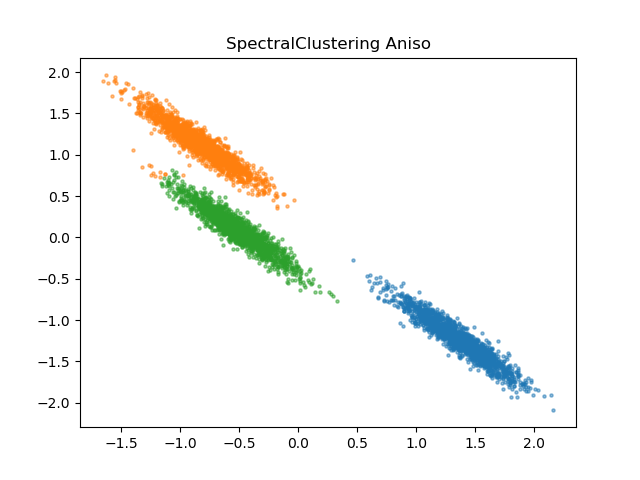
\includegraphics[height=3.5cm]{res/SpectralClustering_Aniso.png}
    \end{minipage}
  }
  \subfigure[Blobs]{
    \begin{minipage}[htbp]{0.3\linewidth}
      \centering
      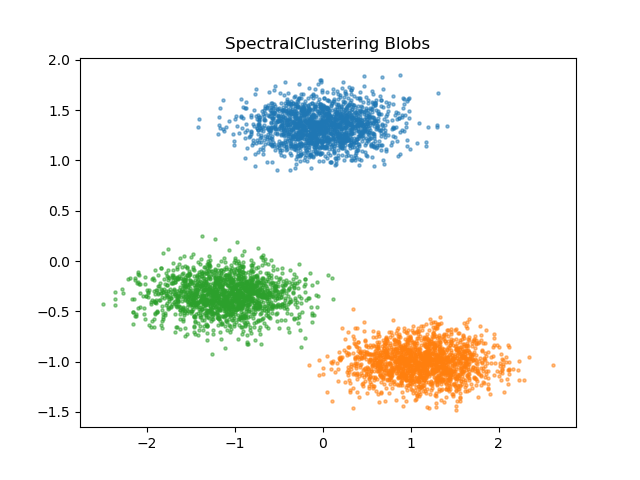
\includegraphics[height=3.5cm]{res/SpectralClustering_Blobs.png}
    \end{minipage}
  }
  \subfigure[Circle]{
    \begin{minipage}[htbp]{0.3\linewidth}
      \centering
      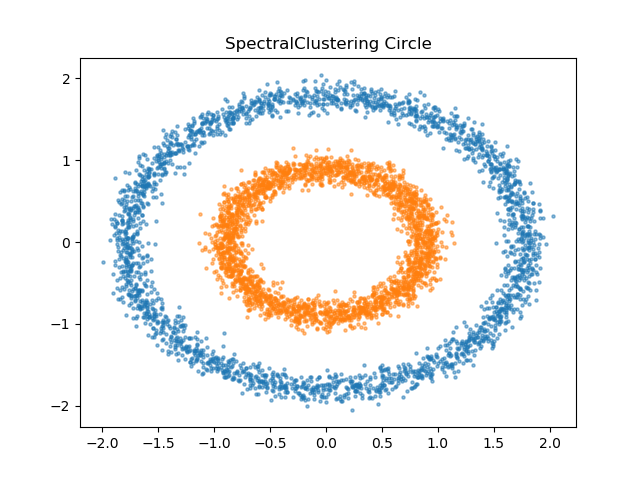
\includegraphics[height=3.5cm]{res/SpectralClustering_Circle.png}
    \end{minipage}
  }

  \subfigure[Moon]{
    \begin{minipage}[htbp]{0.3\linewidth}
      \centering
      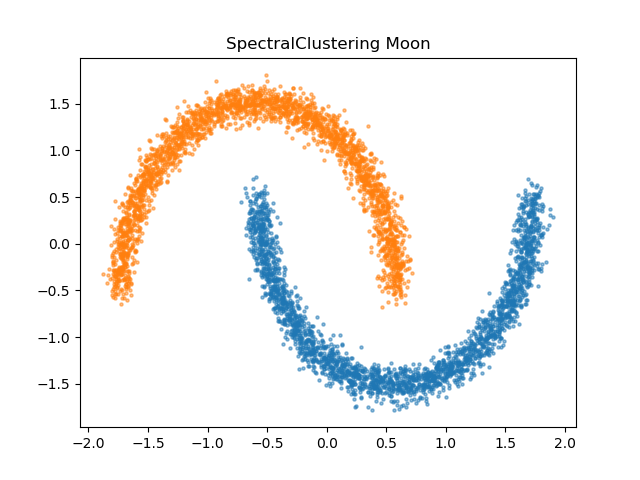
\includegraphics[height=3.5cm]{res/SpectralClustering_Moon.png}
    \end{minipage}
  }
  \subfigure[No Structure]{
    \begin{minipage}[htbp]{0.3\linewidth}
      \centering
      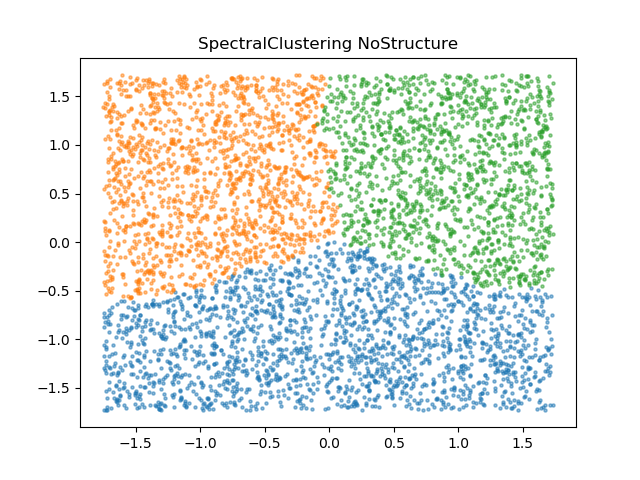
\includegraphics[height=3.5cm]{res/SpectralClustering_NoStructure.png}
    \end{minipage}
  }
  \subfigure[Varied]{
    \begin{minipage}[htbp]{0.3\linewidth}
      \centering
      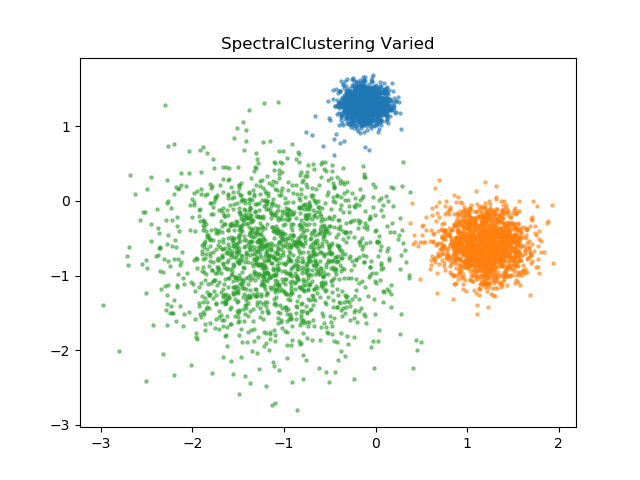
\includegraphics[height=3.5cm]{res/SpectralClustering_Varied.png}
    \end{minipage}
  }
  \caption{Spectral Clustering on Different Datasets}
\end{figure}

\begin{figure}[htbp]
  \centering
  \subfigure[Aniso]{
    \begin{minipage}[htbp]{0.3\linewidth}
      \centering
      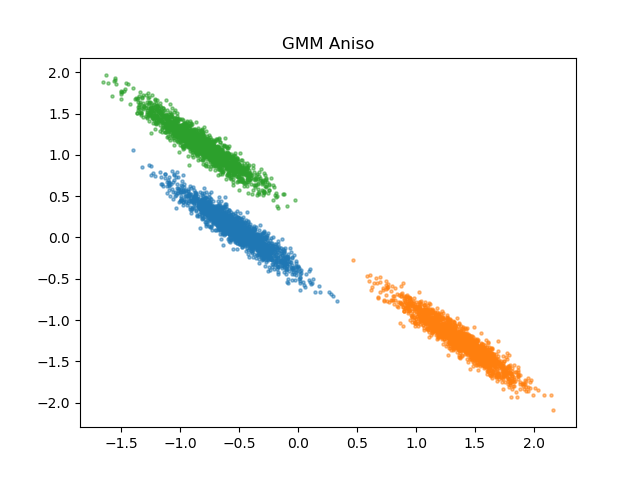
\includegraphics[height=3.5cm]{res/GMM_Aniso.png}
    \end{minipage}
  }
  \subfigure[Blobs]{
    \begin{minipage}[htbp]{0.3\linewidth}
      \centering
      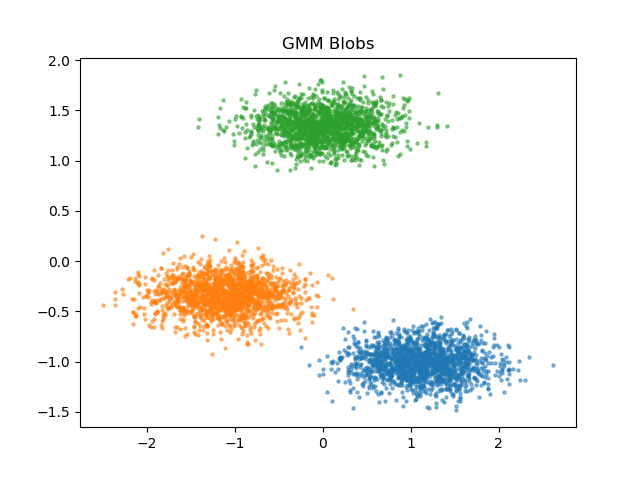
\includegraphics[height=3.5cm]{res/GMM_Blobs.png}
    \end{minipage}
  }
  \subfigure[Circle]{
    \begin{minipage}[htbp]{0.3\linewidth}
      \centering
      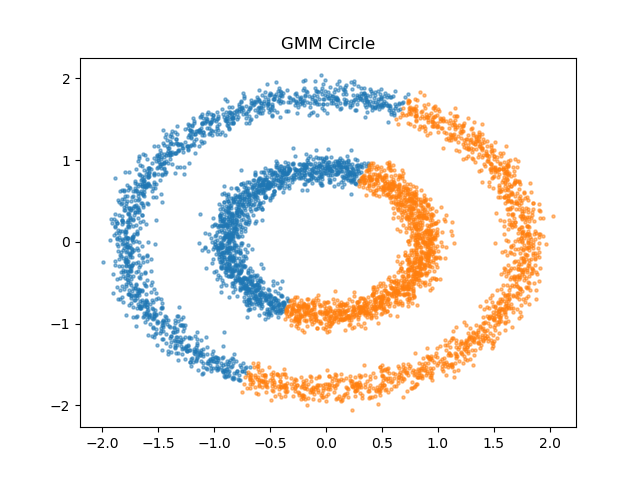
\includegraphics[height=3.5cm]{res/GMM_Circle.png}
    \end{minipage}
  }

  \subfigure[Moon]{
    \begin{minipage}[htbp]{0.3\linewidth}
      \centering
      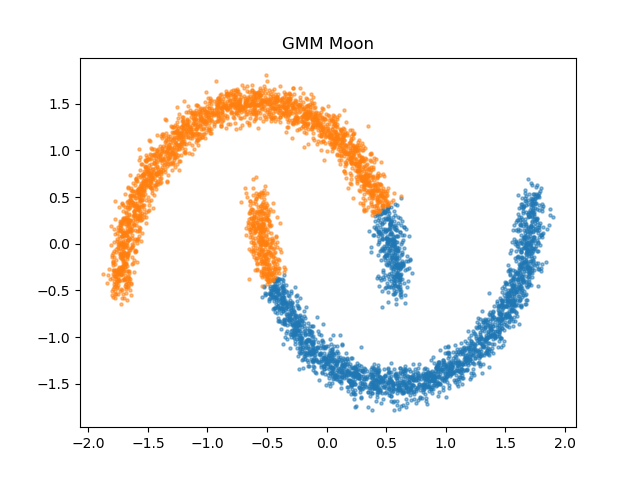
\includegraphics[height=3.5cm]{res/GMM_Moon.png}
    \end{minipage}
  }
  \subfigure[No Structure]{
    \begin{minipage}[htbp]{0.3\linewidth}
      \centering
      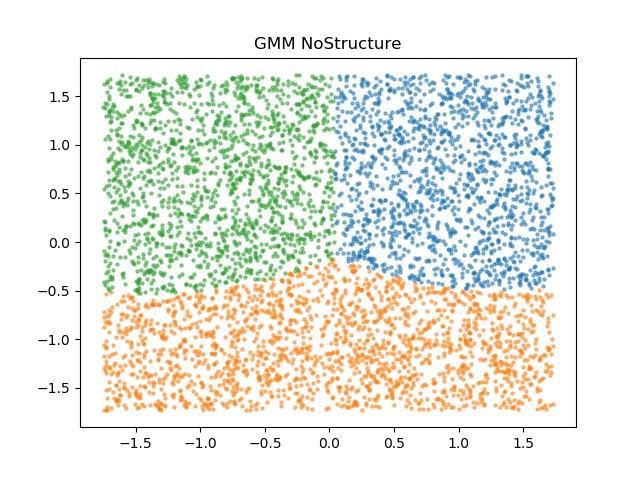
\includegraphics[height=3.5cm]{res/GMM_NoStructure.png}
    \end{minipage}
  }
  \subfigure[Varied]{
    \begin{minipage}[htbp]{0.3\linewidth}
      \centering
      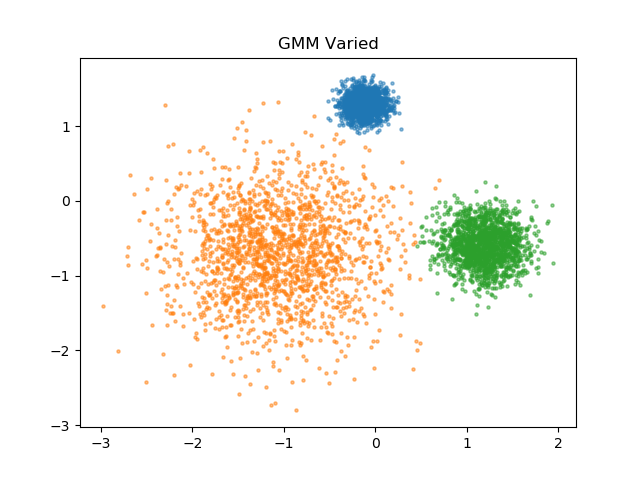
\includegraphics[height=3.5cm]{res/GMM_Varied.png}
    \end{minipage}
  }
  \caption{GMM Clustering on Different Datasets}
\end{figure}

\end{document}